% This is a simple sample document.  For more complicated documents take a look in the exercise tab. Note that everything that comes after a % symbol is treated as comment and ignored when the code is compiled.

\documentclass{article} % \documentclass{} is the first command in any LaTeX code.  It is used to define what kind of document you are creating such as an article or a book, and begins the document preamble

\usepackage{amsmath} % \usepackage is a command that allows you to add functionality to your LaTeX code
\usepackage{amssymb}
\usepackage{tikz}
\usetikzlibrary{calc,matrix}

\title{Tensor Calculus Worksheet!?} % Sets article title
\author{Cheng} % Sets authors name
\date{\today} % Sets date for date compiled

% The preamble ends with the command \begin{document}
\begin{document} % All begin commands must be paired with an end command somewhere
\maketitle % creates title using information in preamble (title, author, date)

\begin{align*}
&Cartesian                      &               &Spherical\\
x(r, \varphi, \theta)&=           &r(x,y,z)&=\\
y(r, \varphi, \theta)&=           &\varphi(x,y,z)&=\\
z(r, \varphi, \theta)&=           &\theta(x,y,z)&=\\
\\
\text{basis}\\
\end{align*}
$$\mathbf{r} = x\hat{x} + y\hat{y} +z\hat{z}  
= x(r, \varphi, \theta)\ \hat{x} +y(r, \varphi, \theta)\ \hat{y} +z(r, \varphi, \theta)\ \hat{z}\\$$
\begin{align*}
\frac{\partial \vec{r}}{\partial x}&=\vec{x}=     &\frac{\partial \vec{r}}{\partial r}&=\vec{r}=\\
\frac{\partial \vec{r}}{\partial y}&=\vec{y}=     &\frac{\partial \vec{r}}{\partial \varphi}&=\vec{\varphi}=\\
\frac{\partial \vec{r}}{\partial z}&=\vec{z}=     &\frac{\partial \vec{r}}{\partial \theta}&=\vec{\theta}=\\
\end{align*}
$$\mathbf{r} = r(x,y,z)\ \vec{r} + \varphi(x,y,z)\ \vec{\varphi} + \theta(x,y,z)\ \vec{\theta}
=r\vec{r} + \varphi \vec{\varphi} + \theta \vec{\theta}$$
\begin{align*}
\frac{\partial \vec{r}}{\partial x}&=\vec{x}=     &\frac{\partial \vec{r}}{\partial r}&=\vec{r}=\\
\frac{\partial \vec{r}}{\partial y}&=\vec{y}=     &\frac{\partial \vec{r}}{\partial \varphi}&=\vec{\varphi}=\\
\frac{\partial \vec{r}}{\partial z}&=\vec{z}=     &\frac{\partial \vec{r}}{\partial \theta}&=\vec{\theta}=\\
\end{align*}

Notice:
$$\frac{\partial \mathbf{r}}{\partial r} = \vec{r} = \partial_r x \ \hat{x} + \partial_r y \ \hat{y} + \partial_r z \ \hat{z}$$

\[
J_{xyz \rightarrow r \varphi \theta} = J^{(xyz)}_{(r\varphi\theta)}=
\frac{\partial(x,y,z)}{\partial(r, \varphi, \theta)} =\\
\begin{bmatrix}
\partial_r x & \partial_{\varphi} x & \partial_{\theta} x\\
\partial_r y & \partial_{\varphi} y & \partial_{\theta} y\\
\partial_r z & \partial_{\varphi} z & \partial_{\theta} z\\
\end{bmatrix}
\]


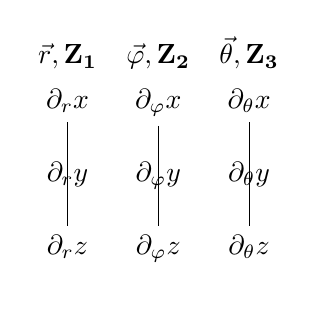
\begin{tikzpicture}[>=stealth]
  \matrix [%
    matrix of math nodes,
    column sep=1em,
    row sep=1em
  ] (Jacobian) {%
  \partial_r x & \partial_{\varphi} x & \partial_{\theta} x\\
  \partial_r y & \partial_{\varphi} y & \partial_{\theta} y\\
  \partial_r z & \partial_{\varphi} z & \partial_{\theta} z\\
  };

  \path (Jacobian-1-1) edge (Jacobian-3-1)
        (Jacobian-1-2) edge (Jacobian-3-2)
        (Jacobian-1-3) edge (Jacobian-3-3);
  {\node[anchor=south] at (Jacobian-1-1.north) {$\vec{r}, \mathbf{Z_1}$};};
  {\node[anchor=south] at (Jacobian-1-2.north) {$\vec{\varphi}, \mathbf{Z_2}$};};
  {\node[anchor=south] at (Jacobian-1-3.north) {$\vec{\theta}, \mathbf{Z_3}$};};
\end{tikzpicture}

\[
J_{r \varphi \theta \rightarrow xyz} = J^{(r\varphi\theta)}_{(xyz)}=
\frac{\partial(r, \varphi, \theta)}{\partial(x,y,z)} =\\
\begin{bmatrix}
\partial_x r       & \partial_y r       & \partial_z r\\
\partial_x \varphi & \partial_y \varphi & \partial_z \varphi\\
\partial_x \theta  & \partial_y \theta  & \partial_z \theta\\
\end{bmatrix}
\]


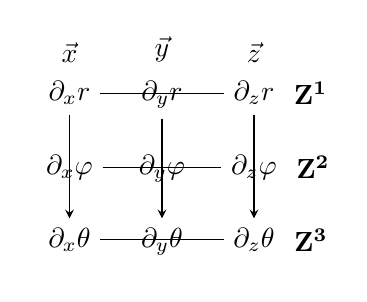
\begin{tikzpicture}[>=stealth]
  \matrix [%
    matrix of math nodes,
    column sep=1em,
    row sep=1em
  ] (Jacobian) {%
  \partial_x r       & \partial_y r       & \partial_z r\\
  \partial_x \varphi & \partial_y \varphi & \partial_z \varphi\\
  \partial_x \theta  & \partial_y \theta  & \partial_z \theta\\
  };

  \path (Jacobian-1-1) edge (Jacobian-1-3)
        (Jacobian-2-1) edge (Jacobian-2-3)
        (Jacobian-3-1) edge (Jacobian-3-3);
  {\node[anchor=west] at (Jacobian-1-3.east) {$\mathbf{Z^1}$};};
  {\node[anchor=west] at (Jacobian-2-3.east) {$\mathbf{Z^2}$};};
  {\node[anchor=west] at (Jacobian-3-3.east) {$\mathbf{Z^3}$};};

  \path (Jacobian-1-1) edge[->] (Jacobian-3-1)
        (Jacobian-1-2) edge[->] (Jacobian-3-2)
        (Jacobian-1-3) edge[->] (Jacobian-3-3);
  {\node[anchor=south] at (Jacobian-1-1.north) {$\vec{x}$};};
  {\node[anchor=south] at (Jacobian-1-2.north) {$\vec{y}$};};
  {\node[anchor=south] at (Jacobian-1-3.north) {$\vec{z}$};};
\end{tikzpicture}

\[
\frac{\partial(r, \varphi, \theta)}{\partial(x,y,z)}
\frac{\partial(x,y,z)}{\partial(r, \varphi, \theta)}
=
\begin{pmatrix}
  1 & 0 & 0 \\
  0 & 1 & 0 \\
  0 & 0 & 1
\end{pmatrix}
=
\begin{pmatrix}
  [\mathbf{Z^1}] \\[0.3cm]
  [\mathbf{Z^2}] \\[0.3cm]
  [\mathbf{Z^3}]
\end{pmatrix}
\begin{pmatrix}
[\mathbf{Z_1}] & [\mathbf{Z_2}] & [\mathbf{Z_3}]
\end{pmatrix}
=
\begin{pmatrix}
  \mathbf{Z^1}\cdot\mathbf{Z_1} & \mathbf{Z^1}\cdot\mathbf{Z_2} & \mathbf{Z^1}\cdot\mathbf{Z_3} \\
  \mathbf{Z^2}\cdot\mathbf{Z_1} & \mathbf{Z^2}\cdot\mathbf{Z_2} & \mathbf{Z^2}\cdot\mathbf{Z_3} \\
  \mathbf{Z^3}\cdot\mathbf{Z_1} & \mathbf{Z^3}\cdot\mathbf{Z_2} & \mathbf{Z^3}\cdot\mathbf{Z_3}
\end{pmatrix}
\]

$$\mathbf{Z^i} \cdot \mathbf{Z_j} = \delta_{ij}$$


%%%%%%%%%%%%%%%%%%%%%%%%%%%%%%%%%%%%%%%%%%%%%%%%%%%%%%%%%%%%%%%%%
\[
\frac{\partial(x,y,z)}{\partial(r, \varphi, \theta)}^T
\frac{\partial(x,y,z)}{\partial(r, \varphi, \theta)}
=
\begin{pmatrix}
  [\mathbf{Z_1}] \\[0.3cm]
  [\mathbf{Z_2}] \\[0.3cm]
  [\mathbf{Z_3}]
\end{pmatrix}
\begin{pmatrix}
[\mathbf{Z_1}] & [\mathbf{Z_2}] & [\mathbf{Z_3}]
\end{pmatrix}
=
\begin{pmatrix}
  \mathbf{Z_1}\cdot\mathbf{Z_1} & \mathbf{Z_1}\cdot\mathbf{Z_2} & \mathbf{Z_1}\cdot\mathbf{Z_3} \\
  \mathbf{Z_2}\cdot\mathbf{Z_1} & \mathbf{Z_2}\cdot\mathbf{Z_2} & \mathbf{Z_2}\cdot\mathbf{Z_3} \\
  \mathbf{Z_3}\cdot\mathbf{Z_1} & \mathbf{Z_3}\cdot\mathbf{Z_2} & \mathbf{Z_3}\cdot\mathbf{Z_3}
\end{pmatrix}
=[Z_{ij}]
\]

%%%%%%%%%%%%%%%%%%%%%%%%%%%%%%%%%%%%%%%%%%%%%%%%%%%%%%%%%%%%%%%
\[
\frac{\partial(r, \varphi, \theta)}{\partial(x,y,z)}
\frac{\partial(r, \varphi, \theta)}{\partial(x,y,z)}^T
=
\begin{pmatrix}
  [\mathbf{Z^1}] \\[0.3cm]
  [\mathbf{Z^2}] \\[0.3cm]
  [\mathbf{Z^3}]
\end{pmatrix}
\begin{pmatrix}
[\mathbf{Z^1}] & [\mathbf{Z^2}] & [\mathbf{Z^3}]
\end{pmatrix}
=
[Z^{ij}]
\]

$$[Z^{ij}][Z_{ij}] =
\frac{\partial(r, \varphi, \theta)}{\partial(x,y,z)}
\frac{\partial(r, \varphi, \theta)}{\partial(x,y,z)}^T
\frac{\partial(x,y,z)}{\partial(r, \varphi, \theta)}^T
\frac{\partial(x,y,z)}{\partial(r, \varphi, \theta)}
=I
$$

$$\therefore Z^{ij}Z_{jk} = \delta_{ik}$$

$$
[Z^{ij}] 
\begin{pmatrix}
  [\mathbf{Z_1}] \\
  [\mathbf{Z_2}] \\
  [\mathbf{Z_3}]
\end{pmatrix}
\overset{?}= 
\begin{pmatrix}
  [\mathbf{Z_1}] \\
  [\mathbf{Z_2}] \\
  [\mathbf{Z_3}]
\end{pmatrix}
$$

$$
[Z^{ij}]
\frac{\partial(x,y,z)}{\partial(r, \varphi, \theta)}^T
=
\frac{\partial(r, \varphi, \theta)}{\partial(x,y,z)}
\frac{\partial(r, \varphi, \theta)}{\partial(x,y,z)}^T
\frac{\partial(x,y,z)}{\partial(r, \varphi, \theta)}^T
=
\frac{\partial(r, \varphi, \theta)}{\partial(x,y,z)}
$$

$$\therefore Z^{ij}\mathbf{Z_j} = \mathbf{Z^i}$$

%%%%%%%%%%%%%%%%%%%%%%%%%%%%%%%%%%%%%%%%%%%%%%%%%%%%%%%%%
Bases:
\begin{align*}
&covariant  &contravariant\\
&\mathbf{Z_1} =  &\mathbf{Z^1} = \\
&\mathbf{Z_2} =  &\mathbf{Z^2} = \\
&\mathbf{Z_3} =  &\mathbf{Z^3} = 
\end{align*}

$$\mathbf{Z^{i}} \cdot \mathbf{Z_j} = \delta^i_j$$

\begin{align*}
&covariant &contravariant\\
\mathbf{V} &= V^i \mathbf{Z_i} &= V_i \mathbf{Z^i}
\end{align*}

\begin{align*}
  \mathbf{V}\cdot\mathbf{V}
  &= covariant \cdot covariant = Z_{ij} V^i V^j \\
  &= covariant \cdot contravariant = \delta_i^{\ j} V^i V_j = V^j V_j\\
  &= contravariant \cdot contravariant = Z^{ij} V_i V_j \\
\end{align*}
\end{document} % This is the end of the document